\documentclass[border=2pt]{standalone}

\usepackage[utf8]{inputenc}
\usepackage{amssymb} % leadsto
\usepackage{tikz}
\usetikzlibrary{positioning,decorations.pathreplacing,matrix,positioning,arrows.meta,arrows,calc}
\tikzset{
mymat/.style={
  matrix of nodes,
  text height=2.5ex,
  text depth=0.75ex,
  text width=3.25ex,
  inner xsep=0ex,
  align=center,
  column sep=-\pgflinewidth,
  nodes={minimum width=4.25ex}
}
}



\begin{document}



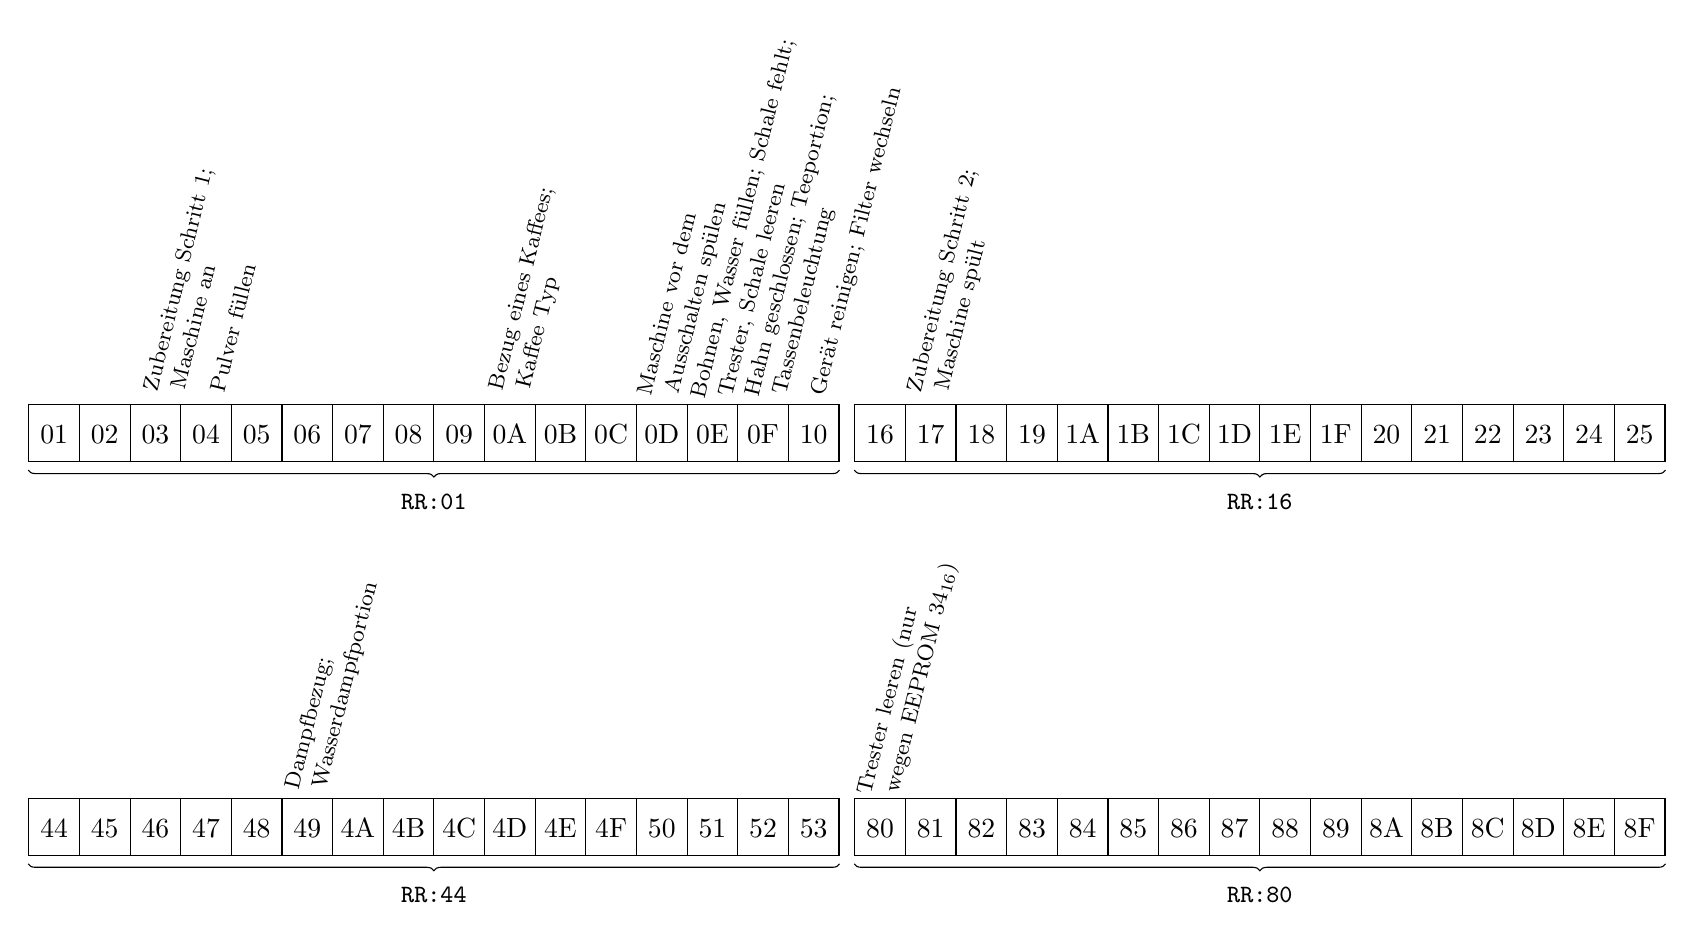
\begin{tikzpicture}[draw, minimum width=1cm, minimum height=0.5cm]
  \matrix[mymat,anchor=west,style={nodes=draw}] at (0,5)
  (Speicher1) {
          |(01)| 01 &
          |(02)| 02 &
          |(03)| 03 &
          |(04)| 04 &
          |(05)| 05 &
          |(06)| 06 &
          |(07)| 07 &
          |(08)| 08 &
          |(09)| 09 &
          |(0A)| 0A &
          |(0B)| 0B &
          |(0C)| 0C &
          |(0D)| 0D &
          |(0E)| 0E &
          |(0F)| 0F &
          |(10)| 10 &
    [2mm]
          |(16)| 16 &
          |(17)| 17 &
          |(18)| 18 &
          |(19)| 19 &
          |(1A)| 1A &
          |(1B)| 1B &
          |(1C)| 1C &
          |(1D)| 1D &
          |(1E)| 1E &
          |(1F)| 1F &
          |(20)| 20 &
          |(21)| 21 &
          |(22)| 22 &
          |(23)| 23 &
          |(24)| 24 &
          |(25)| 25 \\
  };
  
  \matrix[mymat,anchor=west,style={nodes=draw}] at (0,0) 
  (Speicher2) {
          |(44)| 44 &
          |(45)| 45 &
          |(46)| 46 &
          |(47)| 47 &
          |(48)| 48 &
          |(49)| 49 &
          |(4A)| 4A &
          |(4B)| 4B &
          |(4C)| 4C &
          |(4D)| 4D &
          |(4E)| 4E &
          |(4F)| 4F &
          |(50)| 50 &
          |(51)| 51 &
          |(52)| 52 &
          |(53)| 53 &
    [2mm]
          |(80)| 80 &
          |(81)| 81 &
          |(82)| 82 &
          |(83)| 83 &
          |(84)| 84 &
          |(85)| 85 &
          |(86)| 86 &
          |(87)| 87 &
          |(88)| 88 &
          |(89)| 89 &
          |(8A)| 8A &
          |(8B)| 8B &
          |(8C)| 8C &
          |(8D)| 8D &
          |(8E)| 8E &
          |(8F)| 8F \\
  };
  
  \draw[decorate,decoration={brace,mirror,raise=1mm}]
    (01.south west) -- (10.south east) node [black,midway,yshift=-5mm] {\small\texttt{RR:01}};
  \draw[decorate,decoration={brace,mirror,raise=1mm}]
    (16.south west) -- (25.south east) node [black,midway,yshift=-5mm] {\small\texttt{RR:16}};
  \draw[decorate,decoration={brace,mirror,raise=1mm}]
    (44.south west) -- (53.south east) node [black,midway,yshift=-5mm] {\small\texttt{RR:44}};
  \draw[decorate,decoration={brace,mirror,raise=1mm}]
    (80.south west) -- (8F.south east) node [black,midway,yshift=-5mm] {\small\texttt{RR:80}};

  \footnotesize
  \node [above=15.5mm of 03,rotate=76,yshift=-8mm,xshift=1mm,align=left] {Zubereitung Schritt 1;\\\hspace{1mm}Maschine an};
  \node [above=9.5mm of 04,rotate=76,yshift=-5.8mm,xshift=1mm] {Pulver füllen};
  \node [above=14mm of 0A,rotate=76,yshift=-7mm,xshift=1mm,align=left] {Bezug eines Kaffees;\\\hspace{1mm}Kaffee Typ};
  \node [above=13mm of 0D,rotate=76,yshift=-6.5mm,xshift=1mm,align=left] {Maschine vor dem\\\hspace{1mm}Ausschalten spülen};
  \node [above=23.5mm of 0E,rotate=76,yshift=-9.5mm,xshift=1mm,align=left] {Bohnen, Wasser füllen; Schale fehlt;\\\hspace{1mm}Trester, Schale leeren};
  \node [above=20mm of 0F,rotate=76,yshift=-9mm,xshift=1mm,align=left] {Hahn geschlossen; Teeportion;\\\hspace{1mm}Tassenbeleuchtung};
  \node [above=21mm of 10,rotate=76,yshift=-8mm,xshift=1mm,align=left] {Gerät reinigen; Filter wechseln};
  \node [above=15mm of 17,rotate=76,yshift=-7mm,xshift=1mm,align=left] {Zubereitung Schritt 2;\\\hspace{1mm}Maschine spült};
  \node [above=14mm of 49,rotate=76,yshift=-7mm,xshift=1mm,align=left] {Dampfbezug;\\\hspace{1mm}Wasserdampfportion};
  \node [above=15mm of 80,rotate=76,yshift=-7.5mm,xshift=1mm,align=left] {Trester leeren (nur\\\hspace{1mm}wegen EEPROM $34_{16}$)};
\end{tikzpicture}



\end{document}
